\subsection[Демонстрация упрощения реализации компонента управления ресурсами]{Демонстрация упрощения реализации компонента \\ управления ресурсами}

На рис.~\ref{result-before} изображена диаграмма последовательности взаимодействия компонентов системы, в которой нет сервиса управления.
Как видно на диаграмме, в такой системе реализация компонента управления ресурсами (сервиса автомасштабирования) требует реализации получения, обработки и хранения параметров подключения к системе, а так же их последующего использования.
Причём, как видно на диаграмме, сервис автомасштабирования должен уметь обрабатывать различные параметры подключения, специфичные для конкретной платформы виртуализации.
Кроме того, в такой системе сервис автомасштабирования должен содержать реализацию взаимодействия с платформой виртуализации согласно тому программному интерфейсу (API), который она предоставляет.

\begin{figure}[H]
    \centering
    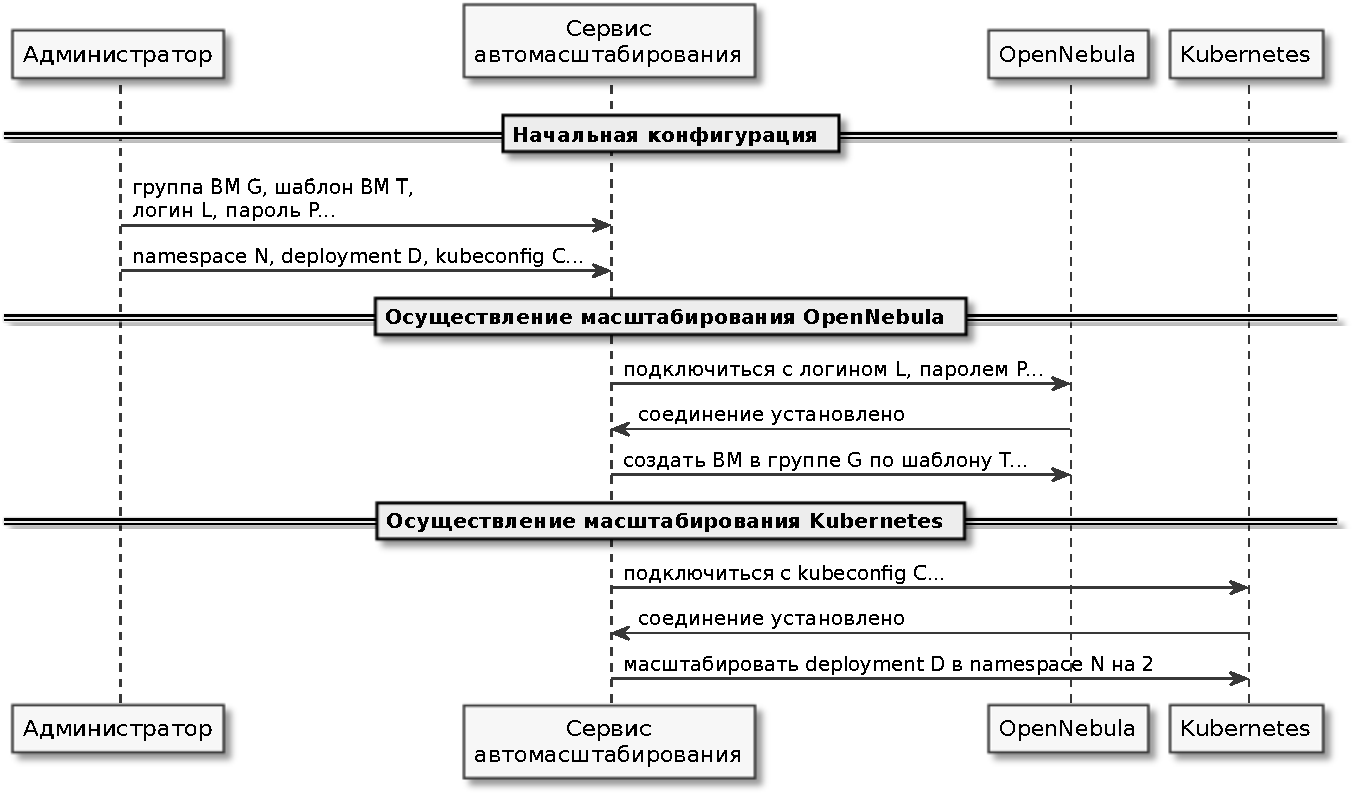
\includegraphics[width=\textwidth]{img/result-before.pdf}
    \caption{Диаграмма последовательности взаимодействия компонентов в системе без сервиса управления}
    \label{result-before}
\end{figure}

Например, платформа OpenNebula оперирует понятиями ''группа ВМ'' и ''шаблон ВМ'', а платформа Kubernetes не использует ВМ совсем, зато использует понятия ''namespace'' и ''deployment'', которых нет в OpenNebula.

С введением в систему сервиса управления, как показано на рис.~\ref{result-after}, взаимодействие с платформами виртуализации и работа администратора не изменились.
Однако реализация компонента управления ресурсами теперь предполагает взаимодействие по одному и тому же унифицированному интерфейсу, не зависящему от используемой платформы виртуализации.
Компонент управления ресурсами должен уметь обрабатывать и хранить только идентификатор управляемого приложения.
Для осуществления самого масштабирования компонент управления теперь не должен уметь оперировать понятиями ''группа ВМ'', ''шаблон ВМ'' и тому подобными.
Напротив, необходимо реализовать лишь команду ''incrementBy'', при получении которой сервис управления сам осуществит горизонтальное масштабирование в соответствии с тем программным интерфейсом, который предоставляет конкретная платформа виртуализации.

\begin{figure}[H]
    \centering
    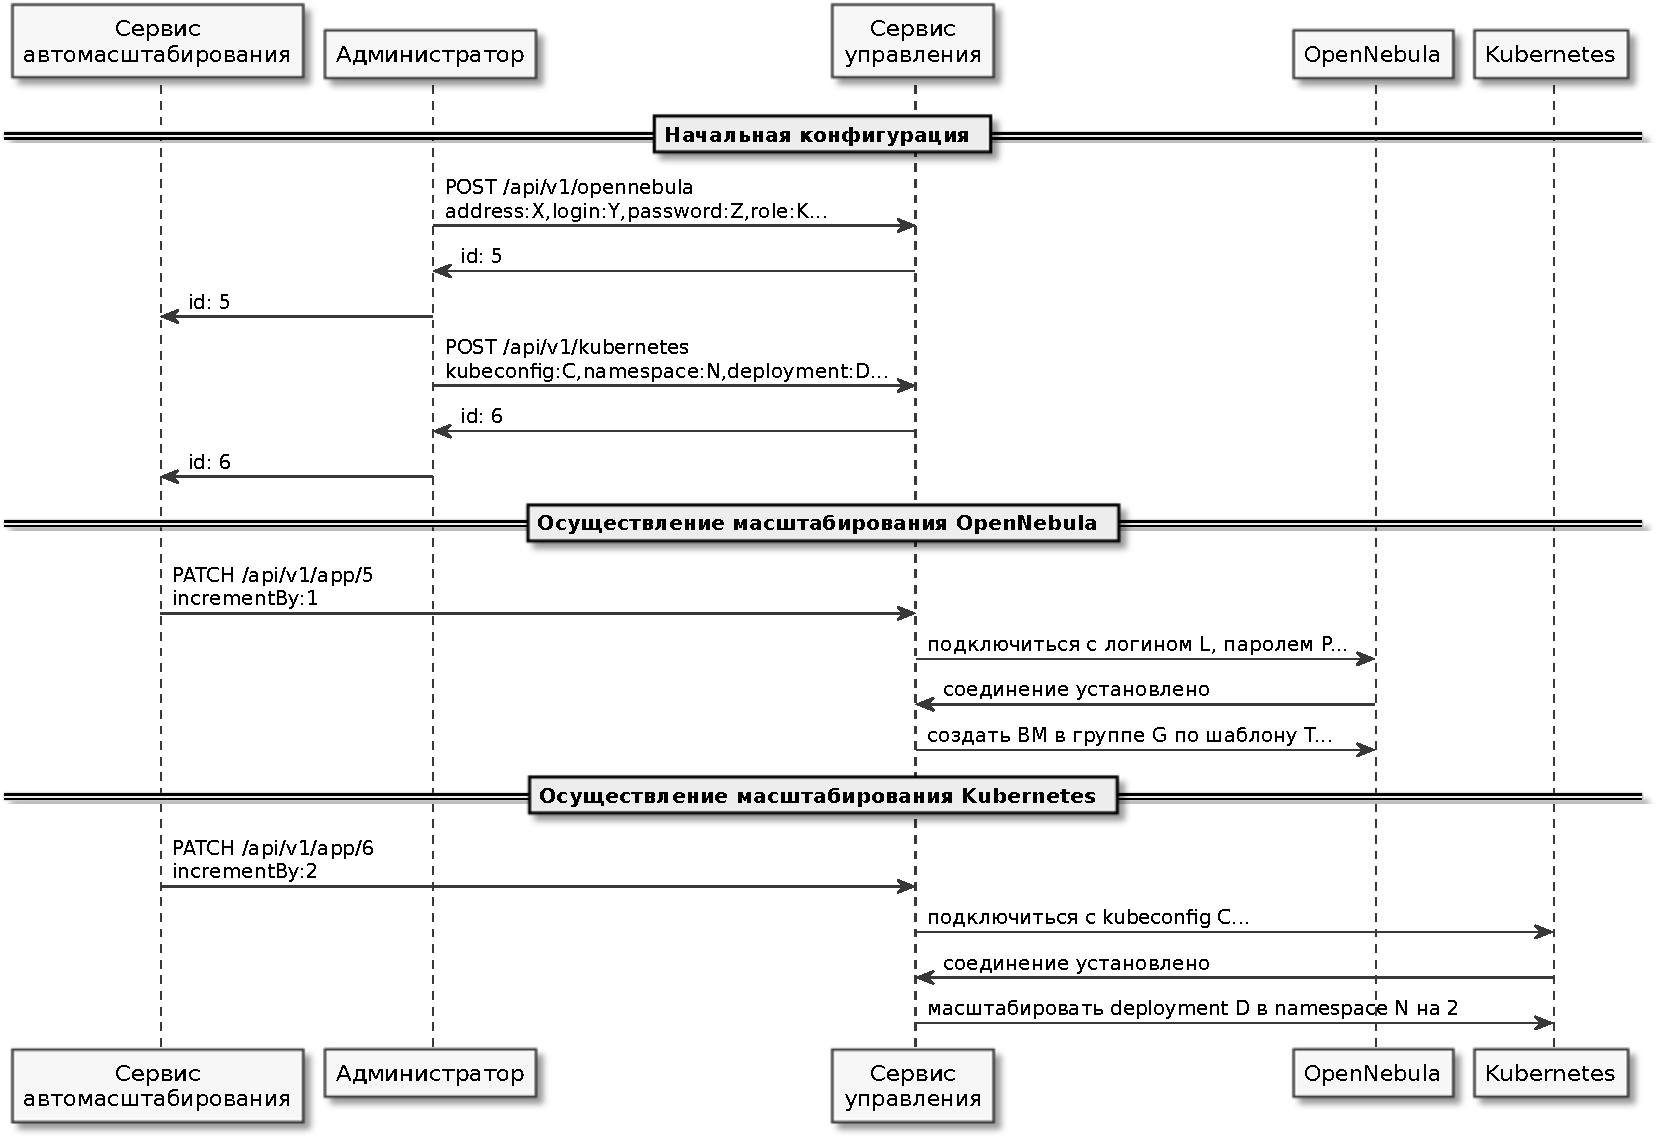
\includegraphics[width=\textwidth]{img/result-after.pdf}
    \caption{Диаграмма последовательности взаимодействия компонентов в системе с сервисом управления}
    \label{result-after}
\end{figure}

Упрощение разработки можно показать с помощью формулы расчёта разницы трудозатрат $T$ на реализацию компонента управления ресурсами (сервиса автомасштабирования) в системе с сервисом управления и в системе без такого сервиса. 

Пусть затраты на реализацию взаимодействия с платформой виртуализации будут $O$, а на реализацию взаимодействия с сервисом управления --- $M$. При этом платформ виртуализации в системе будет предусмотрено $N$, а затраты на реализацию самого компонента управления ресурсами --- $S$.

Предположим также, что зависимость количества трудозатрат на реализацию от количества платформ виртуализации $N$ линейная. 
Тогда затраты $T_1$ на реализацию компонента управления ресурсами в системе без сервиса управления можно рассчитать по формуле~\ref{equ-before}.

\begin{equation}
T_1=S+\sum_{i=1}^{N} O_i
\label{equ-before}
\end{equation}

Трудозатраты $T_2$ на реализацию компонента управления в системе, где предусмотрен сервис управления, можно рассчитать по формуле~\ref{equ-after}.

\begin{equation}
T_2=S+M
\label{equ-after}
\end{equation}

Разницу в трудозатратах $T$ на реализацию компонента управления в системе с сервисом управления и в системе без такого сервиса можно рассчитать по формуле~\ref{equ-compare}.

\begin{equation}
T = T_2 - T_1 = M - \sum_{i=1}^{N} O_i
\label{equ-compare}
\end{equation}

Чем меньше $T$, тем сложнее реализация компонента управления ресурсами без сервиса управления.
В частности, при отрицательных значениях $T$, реализация компонента управления ресурсами в системе с сервисом управления будет проще, чем в такой же системе без него.
